% \chapter{Extending Existing Fingerprinting Methods and Analyzing Entropy}

% In this chapter, our goal is to extend an existing dataset of fingerprints by incorporating browser-based port scanning data and subsequently analyze the resulting changes in entropy. We aim to explore how the addition of browser-based port scanning data enriches our fingerprint dataset and investigate the differences in entropy that emerge as a consequence.

% Our investigation is centered on entropy analysis, a powerful tool for quantifying the level of randomness and diversity within fingerprints. By comparing the entropy of the extended dataset with the original, we seek to uncover whether the integration of port scanning data significantly alters the uniqueness and complexity of the fingerprints.

\chapter{Estimating the Entropy of Browser-Based Port Scanning}

%% \section{Research Objective}

The primary objective of this chapter is to analyze and compare the entropy of synthetic fingerprint datasets under various scenarios. The focus is on understanding how changes in the distribution of open ports and other attributes influence the uniqueness and complexity of fingerprints. 

\subsubsection{Motivation}

The core motivation driving this research is user privacy, particularly user anonymity. As digital fingerprinting techniques continue to advance, the granular details of a user's device, such as the number and identity of open ports, can be key factors in influencing fingerprint complexity. The loss of anonymity, resulting from increased entropy and uniqueness, has potential consequences ranging from unwarranted user profiling to intrusive tracking.

Existing research~\citescientific{gomez2018,laperdrix2016,eckersley2010} has already contributed to determining the entropy of various browser attributes that can be used for fingerprinting. Our objective is to assess the entropy associated with browser-based port scanning, as we believe that browser-based port scanning might be an exceptionally distinctive and often overlooked attribute that can be extracted from a web browser, adding valuable insights to this ongoing research.
Highly unique fingerprints are a threat to user privacy, with the biggest threat being user anonymity. When fingerprints are so distinct that they can be directly linked to specific individuals on a one-to-one basis, the very notion of maintaining anonymity becomes impossible.

Anonymity is important because it provides individuals with a safe way to act, transact, and participate without fear of accountability or reprisal. It encourages freedom of expression, enables people to seek help for stigmatized issues, protects children from online threats, and supports valuable institutions like peer review and whistle-blowing. 
The value of anonymity lies in the ability to remain unreachable, preventing others from demanding explanations or punishments. While in the past, anonymity was often achieved through namelessness, it is the concept of unreachability that is at the heart of its significance, as it safeguards individuals from unwanted consequences and ensures the protection of certain forms of expression and transactions~\citescientific{nissenbaum1999}.

\section{Background}

\subsubsection{Theoretical Limitation}

In theory, the number of possible open port combinations is constrained by the total number of ports available on a system. This results in $2^{65535}$ different combinations.
This number arises from the fact that there are 65,536 ports available on a system, and each of these ports can either be open (1) or closed (0), resulting in a binary representation of open and closed ports for each combination. 
Theoretically, this allows for an immense number of unique port combinations, and thereby a very high entropy.

However, not all ports are detectable by a browser, restricted ports~\citetechnical{firefox_restricted_ports}\citeartifact{chrome_restricted_ports} are not detectable, which is not a significant amount of ports, but still noteworthy.
Additionally, achieving this theoretical limit is neither feasible nor realistic in practice, primarily due to common software usage patterns, limited concurrent applications, and the time it takes to scan the entire port range. 
Moreover, while theoretically, browser-based port scanning could extend to multiple IP addresses, the reality is that fully scanning even a single IP address is already a time-consuming process.
Consequently, we do not consider it realistic to scan multiple IP addresses in a real-world attack.

\subsubsection{Realistic Expectations}
In practice, achieving the full spectrum of possible port combinations is neither practical nor realistic. Several factors contribute to this:

\begin{itemize}
\item One of the primary limitations of browser-based port scanning is the time required for scanning. As previously determined, conducting a scan across the entire port range is a time-consuming process. For instance, on the Chrome browser, it was found that approximately 1,000 ports can be scanned within one second (on Windows). This observation underscores the need for practicality in our approach.

\item To address this limitation, we focus our calculation on a limited number of ports, rather than attempting to scan the entire range of 65,536 ports, we aim to target a limit set of ports, ranging from 1,000 to 10,000 ports, that are associated with the most popular applications and services. However, it is essential to recognize that not all combinations of open ports will occur with the same likelihood.

\item To account for variations in the likelihood of specific port combinations, we employ probability distribution formulas. These formulas will allow us to assign realistic probabilities to each combination of open ports, compared to assigning completely random probabilities. By doing so, we can generate a dataset that somewhat reflects realistic usage patterns, with some applications being more popular than others, while still capturing the diversity of open port combinations. Real-world data would be a better dataset, but this is currently not available.
\end{itemize}

\subsubsection{Probability Distributions}

As we do not have a representative dataset which is large enough to estimate the entropy of browser-based port scanning, we have chosen several probability distributions that seem to align with our limited testing data (n=9) and domain knowledge.
To investigate the relationship between data distribution and fingerprint uniqueness, we have selected three probability distributions to generate synthetic fingerprint datasets: Geometric, Zipf, and Uniform distributions. Each distribution represents different scenarios in terms of port popularity.

\subsubsection{Entropy Calculation}

In order to assess the uniqueness of the different probability distributions, we calculate the entropy of the datasets using Shannon's entropy formula~\citescientific{shannons_entropy}. This formula quantifies the uncertainty or randomness in the dataset and is given by:

\[
H(X) = -\sum_{i=1}^{n} p(x_i) \cdot \log_{2}(p(x_i))
\]

Where:
\begin{itemize}
  \item $H(X)$ represents the entropy of the random variable $X$.
  \item $n$ is the total number of possible outcomes in the random variable $X$.
  \item $p(x_i)$ is the probability of the $i$-th outcome $x_i$.
\end{itemize}

%%\section{Experiment Setup}

\section{Selection of Probability Distributions}

To investigate the relationship between data distribution and fingerprint uniqueness, we have selected three probability distributions to generate synthetic fingerprint datasets: Geometric, Zipf, and Uniform distributions. Each distribution represents different scenarios in terms of port popularity.

\subsubsection{Geometric Distribution}

The Geometric distribution is chosen to model the likelihood of ports being open based on a decreasing geometric progression. This distribution reflects a scenario where some ports are more popular than others, and are therefore more frequently open. The Geometric distribution as depicted in Figures~\ref{fig:geometric_distribution_1000} and~\ref{fig:geometric_distribution_10000}, allows us to simulate a situation where a few ports dominate in terms of usage.

\begin{figure}[h]
\begin{adjustwidth}{-3cm}{-1cm}
\centering
\begin{minipage}{.45\textwidth}
  \centering
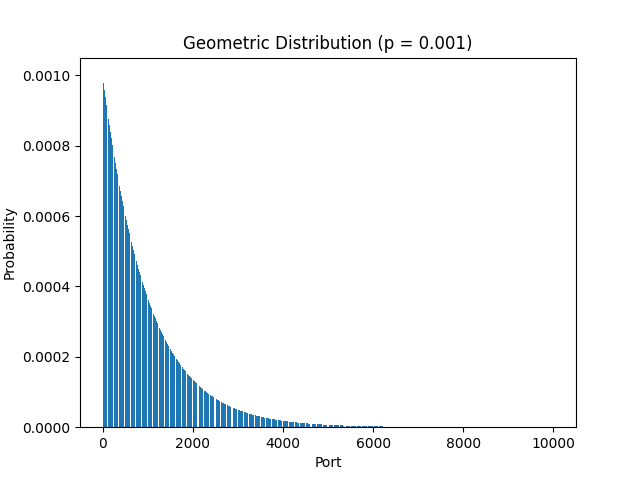
\includegraphics[width=12cm, height=7cm, keepaspectratio]{entropy/img/geometric_distribution_1000.png}
    \caption{Geometric Distribution 1,000 ports}
    \label{fig:geometric_distribution_1000}
\end{minipage}
\hspace{1.5cm}
\begin{minipage}{.45\textwidth}
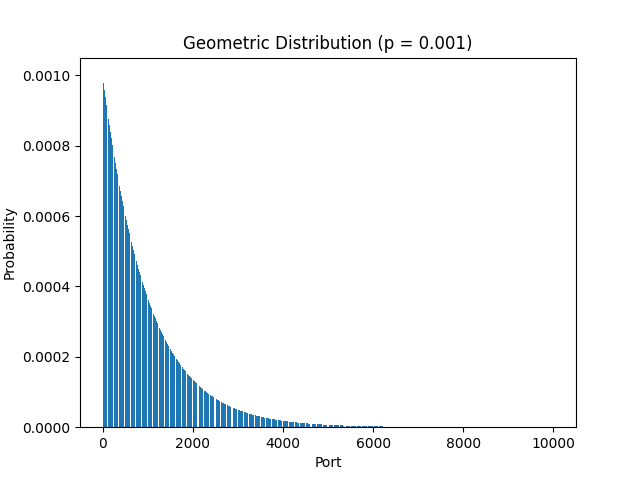
\includegraphics[width=12cm, height=7cm, keepaspectratio]{entropy/img/geometric_distribution_10000.png}
    \caption{Geometric Distribution 10,000 ports}
    \label{fig:geometric_distribution_10000}
\end{minipage}
\end{adjustwidth}
\end{figure}

\subsubsection{Zipf Distribution}

The Zipf distribution is another candidate to represent the distribution of open ports. This distribution is known for modeling scenarios where a small number of items (in our case, ports) are highly popular, while the rest have diminishing popularity. This distribution is useful for simulating scenarios where a small set of ports are commonly open, possibly mirroring common applications and services. This is similar to the geometric distribution, but the distribution is slightly different, which can be seen in the corresponding Figures~\ref{fig:zipf_distribution_1000} and~\ref{fig:zipf_distribution_10000}. 

This distribution aligns the most with our limit dataset. We believe that a distribution resembling the Zipf or Geometric distribution is more plausible in a real-world scenario. This is because certain software applications are more prevalent than others and tend to dominate in terms of usage. Additionally, the fact that many applications cannot be detected through browser-based port scanning further increases the likelihood of these popular applications being even more prevalent.

\begin{figure}[h]
\begin{adjustwidth}{-2cm}{-1cm}
\centering
\begin{minipage}{.45\textwidth}
  \centering
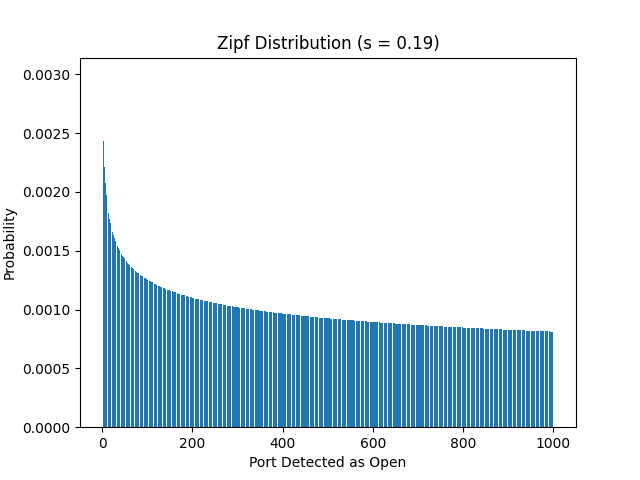
\includegraphics[width=12cm, height=7cm, keepaspectratio]{entropy/img/zipf_distribution_1000.png}
    \caption{Zipf Distribution 1,000 ports}
    \label{fig:zipf_distribution_1000}
\end{minipage}
\hspace{2cm}
\begin{minipage}{.45\textwidth}
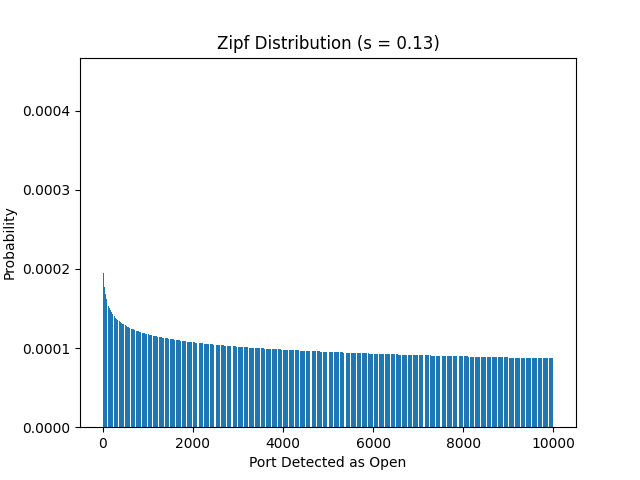
\includegraphics[width=12cm, height=7cm, keepaspectratio]{entropy/img/zipf_distribution_10000.png}
    \caption{Zipf Distribution 10,000 ports}
    \label{fig:zipf_distribution_10000}
\end{minipage}
\end{adjustwidth}
\end{figure}

\subsubsection{Uniform Distribution}

In contrast to the previous two distributions, we include the Uniform distribution to serve as a baseline comparison. In this scenario, all ports are equally likely to be open, which is an unlikely real-world situation but provides insight into what happens to entropy when all ports have equal popularity.

\clearpage
\section{Experiment Setup}

We use a systematic approach to investigate the relationship between data distribution and fingerprint uniqueness. 

\begin{itemize}
\item \textbf{Port Range:} For our experiments, we consider a range of 1,000 and 10,000 ports, representing a subset of the total 65,536 ports available. This choice is based on practical considerations, as scanning all 65,536 ports is time-consuming and not realistic for browser-based port scanning.

\item \textbf{Probability Distribution:} For each of the three selected probability distributions (Geometric, Zipf, Uniform), we calculate the probabilities of individual ports being open based on the chosen distribution. 
\end{itemize}

\subsubsection{Generation of Synthetic Fingerprint Datasets}

In order to properly use Shannon's entropy formula, we have to consider \emph{all possible outcomes}. Calculating all possible outcomes with such a large dataset, i.e. $2^{1000} \approx 1.07 \times 10^{301}$ takes too much time, and therefore we have two possible solutions to calculate entropy:

\begin{itemize}
    \item Sampling from the dataset, i.e. Monte Carlo simulations.
    \item Calculating entropy based on the probability distribution
\end{itemize}

We chose option 2, because sampling from such a large dataset is statistically insignificant, and we can estimate a good average entropy based on the probability distributions.
We use the python NumPy library to calculate the probabilities.

% We begin by generating synthetic fingerprint datasets to serve as the basis for our analysis. To achieve this, we utilize several probability distributions that we estimate to reflect real-world scenarios. These distributions are chosen to simulate various patterns of data distribution. 

% When we refer to data distribution, we are describing the likelihood of each port being open. Certain ports will be detected as open more frequently than others, due to variations in the popularity of the underlying applications. Our goal is to capture this popularity disparity by utilizing different distribution formulas.



\subsubsection{Investigation of Scenario Variations}

We proceed to investigate how different scenarios, represented by variations in the synthetic data, impact the levels of entropy. By introducing changes in the data distribution, we aim to understand how the uniqueness of fingerprints is influenced under various conditions.

\subsubsection{Analysis and Interpretation of Results}

Finally, we analyze and interpret the results obtained from the entropy calculations. Through this analysis, we draw conclusions regarding the relationship between data distribution patterns and the uniqueness of fingerprints. 


% \section{Experiment design}






% \subsection{Entropy Calculation}

% Based on the probabilities of the distributions, we can calculate the entropy using Shannon's entropy formula. This quantifies the uncertainty or randomness in the dataset and provides a measure of fingerprint uniqueness.

% \subsection{Statistical Analysis}

% After conducting the experiments, we perform statistical analysis to identify trends and patterns in the entropy values under various scenarios. We aim to draw conclusions about how changes in data distribution, dataset size, and port range impact fingerprint uniqueness.

% By following this experiment setup, we can gain valuable insights into the relationship between data distribution and the entropy of browser-based port scanning fingerprints, which is crucial for understanding user privacy implications and potential countermeasures.

\section{Results}

In this section, we present the results of our experiments, where we investigated the entropy of synthetic fingerprint datasets generated under different probability distributions: Geometric, Zipf, and Uniform. We varied parameters such as the number of open ports, dataset size, and the range of ports to understand their impact on fingerprint uniqueness.

\subsection{Geometric Distribution}

Under the Geometric distribution, we explored two scenarios:

\subsubsection{Scenario 1: 1,000 Ports}

\begin{itemize}
\item \textbf{Number of Ports Scanned (\(N\)):} 1,000.
\item \textbf{Average Number of Open Ports (\(k\)):} 5.
\item \textbf{Probability of Success (\(p\)):} Calculated as the average number of open ports divided by the total number of ports (\(p = \frac{k}{N}\)).
\end{itemize}

\subsubsection{Scenario 2: 10,000 Ports}

\begin{itemize}
\item \textbf{Number of Ports Scanned (\(N\)):} 10,000.
\item \textbf{Average Number of Open Ports (\(k\)):} 10.
\item \textbf{Probability of Success (\(p\)):} Calculated as the average number of open ports divided by the total number of ports (\(p = \frac{k}{N}\)).
\end{itemize}

With these parameters, the calculated entropy was approximately 9.02 for 1,000 port scans, and 11.41 for 10,000 port scans.

\subsection{Zipf Distribution}

Under the Zipf distribution, we also explored two scenarios:

\subsubsection{Scenario 1: 1,000 Ports}

\begin{itemize}
\item \textbf{Number of Ports Scanned (\(N\)):} 1,000.
\item \textbf{Average Number of Open Ports (\(k\)):} 5.
\item \textbf{Exponent Parameter (\(s\)):} Governs the distribution's skewness. Calculated as \(s \approx \frac{1}{\ln(\frac{N}{k})}\) to achieve a similar level of port popularity as in the Geometric Distribution.
\end{itemize}

\subsubsection{Scenario 2: 10,000 Ports}

\begin{itemize}
\item \textbf{Number of Ports Scanned (\(N\)):} 10,000.
\item \textbf{Average Number of Open Ports (\(k\)):} 10.
\item \textbf{Exponent Parameter (\(s\)):} Governs the distribution's skewness. Calculated as \(s \approx \frac{1}{\ln(\frac{N}{k})}\) to achieve a similar level of port popularity as in the Geometric Distribution.
\end{itemize}

With these parameters, the calculated entropy was approximately 9.93 for 1,000 port scans, and 13.27 for 10,000 port scans.

\subsection{Uniform Distribution}

Under the Uniform distribution, we considered two scenarios:

\subsubsection{Scenario 1: 1,000 Ports}

\begin{itemize}
\item \textbf{Number of Ports Scanned (\(N\)):} 1,000.
\end{itemize}

\subsubsection{Scenario 2: 10,000 Ports}

\begin{itemize}
\item \textbf{Number of Ports Scanned (\(N\)):} 10,000.
\end{itemize}

With these parameters, the calculated entropy was approximately 9.96 for 1,000 ports, and 13.29 for 10,000 ports.


\section{Analysis}

In this section, we analyze the results obtained from the experiment. We compare the differences in entropy when we increase the number of ports scanned (from 1,000 to 10,000) while also taking into account the variations in entropy resulting from different probability distributions. 

\subsubsection{Comparison Between Geometric and Zipf Distributions}

One of the central aspects of the experiment is comparing the Geometric and Zipf distributions in terms of their impact on fingerprint uniqueness. Our findings reveal the following insights: When comparing the Geometric and Zipf distributions, we observe notable differences in the resulting entropy values. Under similar scenarios, the Zipf distribution consistently yields higher entropy compared to the Geometric distribution. This demonstrates the impact of distribution skewness on fingerprint complexity. 

As logically follows, due to the Zipf distribution being more uniform than the Geometric distribution, the uniqueness of the Zipf distribution is higher. This means that if the popularity of certain applications is not as prevalent as we think it is, the entropy will be even more unique. Nevertheless, the Geometric distribution already gives 9 bits of entropy within 1 second of port scanning (1,000 ports).

\subsubsection{Impact of Increased Search Space}

Another aspect we explored is the influence of expanding the search space by increasing the number of ports scanned.
For the Geometric distribution, transitioning from scanning 1,000 ports with 5 average open ports (Scenario 1) to scanning 10,000 ports with 10 average open ports (Scenario 2) resulted in a relatively modest increase in entropy, approximately 2.39 bits. This suggests that, for the Geometric distribution, the search space expansion had a more incremental effect on fingerprint uniqueness.
In contrast, the Zipf distribution exhibited a more substantial impact when transitioning between scenarios. The entropy increased by approximately 3.34 bits, emphasizing that the Zipf distribution's effectiveness in generating unique fingerprints becomes more pronounced with a larger search space.

On certain webpages where a user is expected to stay for a longer time, the search space can be expanded to a higher number. When 1,000 ports are mapped to the most popular applications currently opening a port, browser-based port scanning becomes a realistic and powerful fingerprinting technique. Especially when ports outside the dynamic port range are scanned, browser-based port scanning can be utilized for user-tracking, as most ports will not be ephemeral.

It is important to emphasize that while a user is navigating a website, browser-based port scanning can continue without interruption. A sophisticated scanning mechanism can efficiently scan, and at the same time, relay the scan results back to a server. This extends the scanning duration throughout the user's entire session on the website, which typically lasts much longer than one second. As a result, the search space can easily be expanded to accommodate up to 10,000 ports or higher, depending on the website. The larger the search space, the higher the entropy will be.

\subsubsection{Uniform Distribution Comparison}

We also compared the Uniform distribution with both distributions.
Notably, the Uniform distribution exhibited similar entropy values to the Zipf distribution under similar scenarios, despite the difference in the probability of detecting open ports.

\subsubsection{Real world validation}

We have integrated browser-based port scanning~\citeartifact{fpjspr} within the popular FingerprintJS library~\citeartifact{fingerprintjs}, and we assessed that 1,000 ports can easily be scanned on any webpage, together with existing fingerprinting techniques, without noticeable impact on the end user. 


\section{Conclusion}

In conclusion, our experiments show that browser-based port scanning is a realistic threat to user anonymity on the internet, based on our assumptions. We have examined the impact of different probability distributions (Geometric, Zipf, and Uniform) and the expansion of search space on the entropy of fingerprints generated through port scanning.
One of the most important findings of this experiment is that regardless of the distribution used, we consistently observed high levels of entropy, indicating the potential for creating highly unique fingerprints through browser-based port scanning, within a short period of scanning time (< 1 second).

This finding suggests that a fingerprint with an entropy of at least 9 can be generated within roughly one second of scanning. When combined with existing fingerprinting techniques, such as time zone, plugins, ad blocker, user-agent, fonts, screen resolution, etc., this results in a cumulative entropy that exceeds 29 bits of entropy~\citescientific{gomez2018}. Narayanan~\citescientific{narayanan201233} argues that an entropy of 33 bits is sufficient to uniquely identify users ($2^{33}$ = 8,59 billion), an entropy that is realistic if the search space is large enough, emphasizing the threat that browser-based port scanning poses to user anonymity on the internet.

In light of these findings, it is evident that browser-based port scanning can be a tool for user profiling and tracking, especially when combined with existing fingerprinting techniques. As such, it is imperative for users, and more importantly browser developers, to be aware of these threats and take proactive measures to prevent unauthorized local port scanning.







% \begin{enumerate}
%   \item \textbf{Common Software Usage:} Most users run common software applications that open specific ports. This commonality reduces the variation in open port combinations.
  
%   \item \textbf{Limited Concurrent Applications:} Users typically run a limited number of applications simultaneously, further reducing the number of open ports that can be detected.
  
%   \item \textbf{Port Popularity:} Certain ports, such as those associated with popular services (e.g., email, web browsing, and messaging), are more frequently open, while others remain closed by default.
% \end{enumerate}



% https://math.stackexchange.com/questions/2729561/probability-of-an-unordered-sample-under-weighted-sampling-without-replacement




% https://dl.acm.org/doi/fullHtml/10.1145/3178876.3186097